
\documentclass{article}

\usepackage{tikz}
\usetikzlibrary{mindmap,trees}
\usepackage[margin=0pt,hmargin={-0.5cm,0cm},papersize={14.85cm,11cm}]{geometry} 
\begin{document}
\pagestyle{empty}



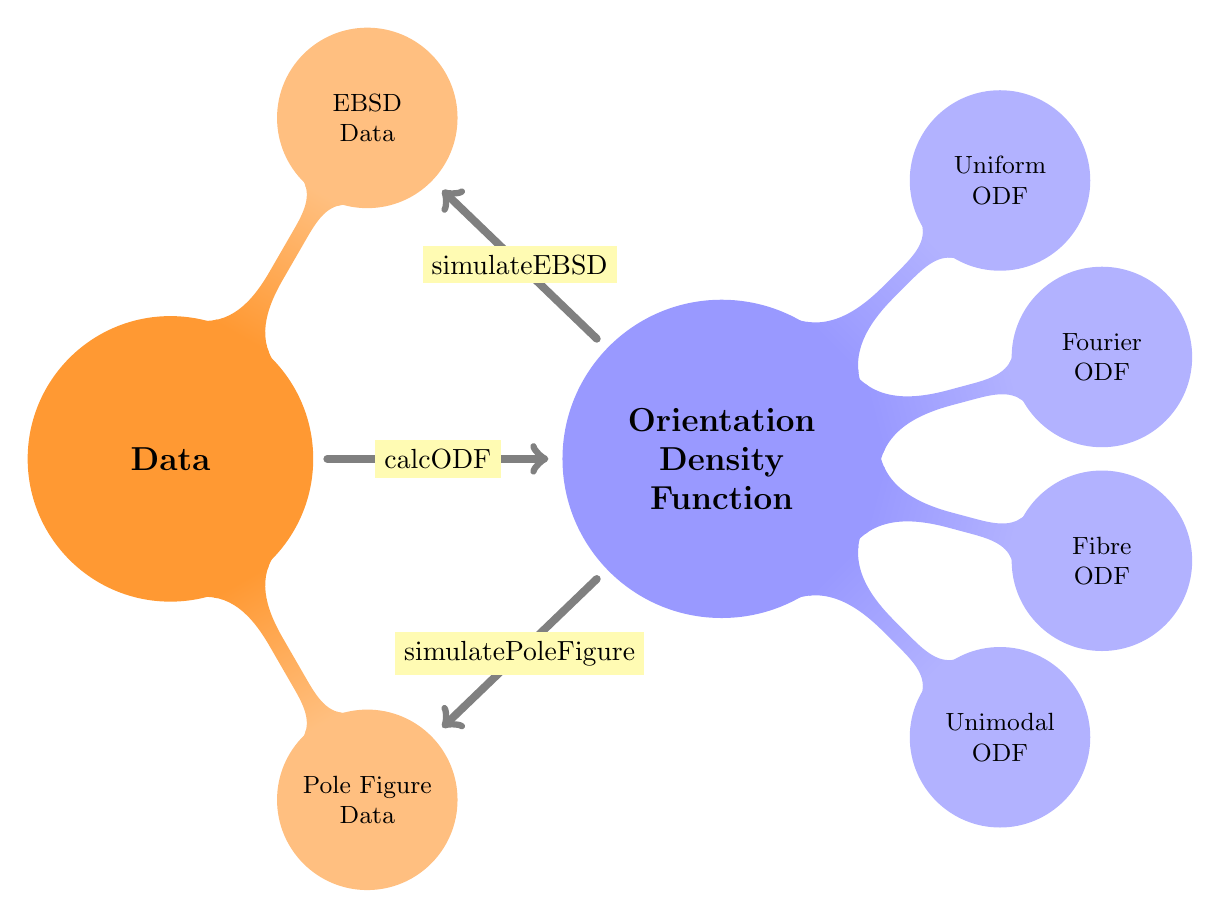
\begin{tikzpicture}[scale = 1]
  \definecolor{myblue}{HTML}{92dcec}
  \tikzstyle{every annotation}=[fill=white, font=\sf]

  \path[mindmap, concept color=orange!80!]
  node[concept,minimum size=3cm](data) at (-7,0) {\bf Data} 
  child[grow = 60, concept color=orange!50] 
  { node(ebsd) [concept](ebsd2) {EBSD \\
      Data} }
  child[grow = -60, concept color=orange!50] 
  { node[concept](pf) {Pole Figure\\Data}};

  \path[mindmap,concept color=blue!40!]
  node[concept](odf) {\bf Orientation Density Function}
%  [clockwise from=0]
  child[grow = -45, concept color=blue!30!] 
  { node [concept](zwei) {Unimodal \\ ODF} }
  child[grow = -15, concept color=blue!30] { node[concept] {Fibre \\ ODF}}
  child[grow = 15, concept color=blue!30] { node [concept] {Fourier \\
      ODF}}
 child[grow = 45, concept color=blue!30] { node [concept] {Uniform\\
      ODF}};


  \draw [->,concept connection] (odf) edge 
  node[fill=yellow!30] {simulateEBSD}  
  (ebsd2);
  ; 
  \draw [->,concept connection] (odf) edge 
  node[fill=yellow!30] {simulatePoleFigure}  (pf);
  \draw [<-,concept connection] (odf) edge 
  node[fill=yellow!30] {calcODF}  
  (data);

%  \path[mindmap, concept color=orange!80!]
%  node[concept,minimum size=3cm](data) at (3,-3) {\bf Visualization} 
%  child[grow = 60, concept color=orange!50] 
%  { node(ebsd) [concept](ebsd2) {EBSD \\
%      Data} }
%  child[grow = -60, concept color=orange!50] 
%  { node[concept](pf) {Pole Figure\\Data}};



%  \node[ below] at (ebsd.south){calcODF; simulateEBSD};
%node[above,very near start] {incoming beam};
\end{tikzpicture}
\end{document}
%%% Local Variables: 
%%% mode: latex
%%% TeX-master: t
%%% End: 
